\documentclass[11pt,a4paper]{article}
\usepackage{gtu-el-yazisi}
\begin{document}
\notbilgi{Alan Teorisi}{Final çalışma notu (Uygulama ve Ders notları)}{Final-notu-kopya.pdf}

\sayfa{1}
\section{Uygulama 7 -- İç içe iki küre}

\begin{center}
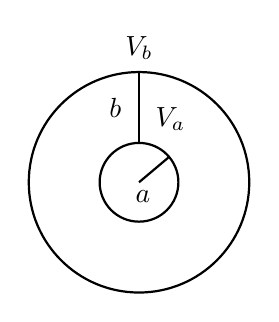
\begin{tikzpicture}[line width=0.8pt]
  \draw (0,0) circle (1.4);
  \draw (0,0) circle (0.5);
  \draw (0,1.4) -- (0,0.5);
  \draw (0,0) -- (0.38,0.32);
  \node at (-0.3,0.95) {$b$};
  \node at (0,1.7) {$V_b$};
  \node at (0.4,0.8) {$V_a$};
  \node at (0.05,-0.18) {$a$};
\end{tikzpicture}
\end{center}

$a<r<b$ \qquad $V(r)=\dfrac{V_a-V_b}{\dfrac1a-\dfrac1b}\cdot\dfrac1r+\dfrac{aV_a-bV_b}{a-b}$

$r<a$ \quad $\vec E=0$ \quad (içerde yük yok)

$\vec E=-\mathrm{grad}\,V \xrightarrow{\text{integral}} V(r)=C$ olur

\[ V(a)=V_a=C \;\Rightarrow\; \kutula{r<a\ \ V(r)=V_a} \]

$r>b$ \quad $\Delta V=0$ \quad $\dfrac{1}{r^2}\dfrac{\partial}{\partial r}\!\left(r^2\dfrac{\partial V}{\partial r}\right)=0$

\[ r^2\frac{\partial V}{\partial r}=-A \;\Rightarrow\; \frac{\partial V}{\partial r}=-\frac{A}{r^2} \]
\[ V(r)=\frac{A}{r}+B \]

$r\to\infty$ \ $V(r)=0$ olmalıdır $\Rightarrow B=0$

$r=b$ \quad $V(b)=V_b=\dfrac{A}{b}\ \Rightarrow\ A=bV_b$

\[ V(r)=\frac{bV_b}{r} \]

O zaman

\begin{align*}
a<r<b\quad \vec E=-\mathrm{grad}\,V&=\frac{V_a-V_b}{\dfrac1a-\dfrac1b}\,\frac{1}{r^2}\,\vec e_r\\
r<a\quad \vec E&=0\\
r>b\quad \vec E=-\mathrm{grad}\,V&=-\frac{\partial}{\partial r}\!\left(\frac{bV_b}{r}\right)\vec e_r=\frac{bV_b}{r^2}\,\vec e_r
\end{align*}

\[ r=a\text{ da}\quad \kutula{\vec E=\frac{\vec E^{+}(a)+\vec E^{-}(a)}{2}} \]

\begin{align*}
&=\frac12\left[\frac{V_a-V_b}{\dfrac1a-\dfrac1b}\cdot\frac{1}{a^2}\right]\vec e_r\\[2mm]
&=\frac12\,\frac{b}{a}\left[\frac{V_a-V_b}{b-a}\right]\vec e_r
\end{align*}

\textcolor{kirmizikalem}{$a$ yüzeyindeki yüke etkiyen kuvvet??}

\vurgu{$d\vec{F}=\rho_s\,ds\,\vec{E}$} \qquad \vurgu{$ds=a^2\sin\theta\,d\phi\,d\theta$}

\vurgu{$\mathrm{div}\,\vec{D}=\rho_s$}

\formulkutu[sınır koşulu]{\rho_s=\vec n\cdot\vec D=\vec n\cdot\varepsilon\vec E=\vec e_r\cdot\varepsilon\cdot\vec E}

$a$ noktasında
\[ \rho_s=\varepsilon\cdot\frac12\cdot\frac{b}{a}\left[\frac{V_a-V_b}{b-a}\right] \]

\section{Ders 9 -- Değişik türden yük dağılımları ve Dirac Distribüsyonu}

\noindent hacimsel $\rho_v\ [\mathrm{C/m^3}]$ \hfill yüzeysel $\rho_s\ [\mathrm{C/m^2}]$ \hfill çizgisel $\rho_c\ [\mathrm{C/m}]$

\elcizimi[0.4]{sekiller/final-calismasi-Final-notu-kopya-s1-1.png}[1]

$\rho_s(y,z)$ \quad $x=0$'da $\rho_s(y,z)\ [\mathrm{C/m^2}]$ yük yoğunluğu olsun; bu yüzeysel yük yoğunluğuna ilişkin hacimsel yük yoğunluğu:
\[ \underset{[\mathrm{C/m^3}]}{\rho_v(x,y,z)}=\underset{[\mathrm{C/m^2}]}{\rho_s(y,z)}\,\underset{[1/\mathrm{m}]}{\delta(x)} \]

\subsection{$\delta(x)$'in özellikleri}
\begin{enumerate}
\item $a\le x\le b,\ c\le y\le d,\ e\le z\le f$ prizması içindeki toplam yük $\bigl(\rho_v(x,y,z)=\rho_s(y,z)\,\delta(x)\bigr)$
\[ Q=\int\limits_{x=a}^{b}\int\limits_{y=c}^{d}\int\limits_{z=e}^{f}\rho_v(x,y,z)\,dx\,dy\,dz \]
\[ Q=\int\limits_{x=a}^{b}\int\limits_{y=c}^{d}\int\limits_{z=e}^{f}\rho_s(y,z)\,\delta(x)\,dx\,dy\,dz \]
\[ =\int\limits_{x=a}^{b}\delta(x)\,dx\int\limits_{y=c}^{d}\int\limits_{z=e}^{f}\rho_s(y,z)\,dy\,dz \]
\[ \Rightarrow\ \begin{cases} a,b<0,\ Q=0\\ a,b>0,\ Q=0\\ a<0<b,\ Q=\displaystyle\int\limits_{y=c}^{d}\int\limits_{z=e}^{f}\rho_s(y,z)\,dy\,dz\end{cases} \]
çünkü $\displaystyle\int\limits_{x=a}^{b}\delta(x)\,dx=\begin{cases}0, & ab>0\\ 1, & a<x<b\end{cases}$\footnote{Claude notu: muhtemelen $a<0<b$ olmalı.}
\item $g(x)\,\delta(x)=g(0)\,\delta(x)$
\item $\displaystyle\int\limits_{a}^{b}\delta(x)\,dx=\begin{cases}0, & ab>0\\ 1, & a<x<b\end{cases}$

$a\to-\infty,\ b\to x$
\[ \int\limits_{-\infty}^{x}\delta(x)\,dx=\begin{cases}0, & x<0\\ 1, & x>0\end{cases}=u(x)\ \text{ birim basamak fonksiyonu} \]
\end{enumerate}
\formulkutu{\delta(x)=\dfrac{\partial u(x)}{\partial x}}

\sayfa{2}
\begin{gather*}
d\vec F=\rho_s\,ds\,\vec E_{\mathrm{orta}}\\
d\vec F=\frac{\varepsilon}{2}\,\frac{b}{a}\left[\frac{V_a-V_b}{b-a}\right]\left(a^2\sin\theta\,d\phi\,d\theta\right)\\
\left[\frac12\,\frac{b}{a}\left(\frac{V_a-V_b}{b-a}\right)\vec e_r\right]\\
\vec F=\int\limits_{\theta=0}^{\pi}\int\limits_{\phi=0}^{2\pi}\frac{\varepsilon}{4}\,b^2\left[\frac{V_a-V_b}{b-a}\right]^{2}\sin\theta\,d\phi\,d\theta\ \vec e_r\\
\vec F=\varepsilon\pi b^2\left(\frac{V_a-V_b}{b-a}\right)^{2}\vec e_r
\end{gather*}

$r=b$ için\footnote{Claude notu: Orijinalde bu satırlardaki bazı $b$ çarpanları sadeleştirme için çizilmiştir (sayfa 2'nin sol sütununda birkaç yerde).}
\[ \vec E=\frac{\vec E^{+}(b)+\vec E^{-}(b)}{2} \]
\begin{align*}
&=\frac12\left[\frac{bV_b}{b^2}+\frac{ab}{b^2}\left(\frac{V_a-V_b}{b-a}\right)\right]\\[2mm]
&=\frac12\left[\frac{V_b(b-a)+a(V_a-V_b)}{b(b-a)}\right]\\[2mm]
&=\frac{bV_b-2aV_b+aV_a}{2b(b-a)}\,\vec e_r
\end{align*}

\begin{gather*}
\rho_s=\varepsilon\cdot\vec n\cdot\vec E=\varepsilon\,\vec e_r\,\vec E\\
\rho_s=\frac{\varepsilon}{2b(b-a)}\left[bV_b-2aV_b+aV_a\right]\\
ds=b^2\sin\theta\,d\theta\,d\phi\\
d\vec F=\rho_s\,ds\,\vec E
\end{gather*}
\begin{align*}
&=\frac{\varepsilon}{2b(b-a)}\left[bV_b-2aV_b+aV_a\right]\left(b^2\sin\theta\,d\theta\,d\phi\right)\\
&\quad\cdot\left[\frac{bV_b-2aV_b+aV_a}{2b(b-a)}\right]\vec e_r
\end{align*}
\[ \vec F=\int\limits_{\theta=0}^{\pi}\int\limits_{\phi=0}^{2\pi}d\vec F \]
\[ =\varepsilon\pi\left[\frac{bV_b-2aV_b+aV_a}{b-a}\right]^{2}\vec e_r \]

\begin{enumerate}[start=2]
\item \elcizimi[0.55]{sekiller/final-calismasi-Final-notu-kopya-s2-1.png}[2]
\end{enumerate}

\begin{enumerate}[start=4]
\item
\begin{center}
\begin{tikzpicture}[line width=0.8pt]
  \draw[-{Stealth}] (-3.3,0) -- (3.4,0) node[right] {$x$};
  \draw[-{Stealth}] (0,-0.7) -- (0,3.0) node[right] {$f(x)$};
  \node at (0.5,-0.35) {$x=0$};
  \draw[murekkep] (-3.2,1.2) .. controls (-2.2,1.3) and (-1.2,1.1) .. (0,1.2);
  \draw[murekkep] (0,2.1) .. controls (1.0,2.2) and (2.2,2.0) .. (3.2,2.1);
  \node at (-1.6,0.85) {$f_-(x)$};
  \node at (2.6,2.5) {$f_+(x)$};
  \node at (0.4,1.65) {$\left.\vphantom{\rule{0pt}{7mm}}\right\}\,\Delta f$};
\end{tikzpicture}
\end{center}
\[ f(x)=\begin{cases} f_-(x), & x<0\\ f_+(x), & x>0\end{cases} \]
$x=0$'da süreksizlik var
\[ f(x)=f_+(x)\,u(x)+f_-(x)\,u(-x) \]
\begin{align*}
f'(x)&=f'_+(x)\,u(x)+\underbrace{f_+(x)\,\delta(x)}_{f_+(0)\,\delta(x)}+f'_-(x)\,u(-x)\\
&\quad\underbrace{-f_-(x)\,\delta(x)}_{f_-(0)\,\delta(x)}
\end{align*}
\begin{align*}
f'(x)&=\overbrace{\left[f'_-(x)\,u(-x)+f'_+(x)\,u(x)\right]}^{\{f'(x)\}}\\
&\quad+\underbrace{\left[f_+(0)-f_-(0)\right]\delta(x)}_{[|f|]\,\delta(x)}
\end{align*}
\[ f'(x)=\underbrace{\{f'(x)\}}_{\text{Regüler kısım}}+\underbrace{[|f|]\,\delta(x)}_{\text{Tekil (singüler kısım)}} \]

\[ \mathrm{grad}\,V=\frac{\partial V}{\partial x}\vec e_x+\frac{\partial V}{\partial y}\vec e_y+\frac{\partial V}{\partial z}\vec e_z \]
$x=0$'da bir süreksizlik olsun
\begin{gather*}
\frac{\partial V}{\partial x}=\left\{\frac{\partial V}{\partial x}\right\}+\left[|V\vec e_x|\right]\delta(x)\\
\frac{\partial V}{\partial y}=\left\{\frac{\partial V}{\partial y}\right\}\\
\frac{\partial V}{\partial z}=\left\{\frac{\partial V}{\partial z}\right\}
\end{gather*}
\elcizimi[0.28]{sekiller/final-calismasi-Final-notu-kopya-s2-2.png}[2]

$V$'nin süreksizliği herhangi bir $S$ yüzeyi üzerinde olsaydı
\elcizimi[0.22]{sekiller/final-calismasi-Final-notu-kopya-s2-3.png}[2]
\[ \mathrm{grad}\,V=\{\mathrm{grad}\,V\}+\left[|V\hat n|\right]\delta(s) \]

\item $x=0$'da süreksizliği olan $\vec E(x,y,z)$ için
\[ \mathrm{div}\,\vec E=\frac{\partial E_x}{\partial x}+\frac{\partial E_y}{\partial y}+\frac{\partial E_z}{\partial z} \]
\begin{gather*}
\frac{\partial E_x}{\partial x}=\left\{\frac{\partial E_x}{\partial x}\right\}+\left[|E_x|\right]\delta(x)\\
\frac{\partial E_y}{\partial y}=\left\{\frac{\partial E_y}{\partial y}\right\}\,,\qquad\frac{\partial E_z}{\partial z}=\left\{\frac{\partial E_z}{\partial z}\right\}
\end{gather*}
\end{enumerate}

\sayfa{3}
$a<\rho<b$
\[ V(\rho)=\frac{V_a-V_b}{\ln a-\ln b}\,\ln\rho-\frac{V_a\ln b-V_b\ln a}{\ln a-\ln b} \]

$\rho<a$ \quad $\vec E=0,\ \vec E=-\mathrm{grad}\,V\Rightarrow V(\rho)=C$ ($\to$ sabit)

$\Rightarrow V(\rho)=V_a$

$\rho>b$ \quad $\Delta V=0$
\[ \frac1\rho\frac{\partial}{\partial\rho}\left(\rho\frac{\partial V}{\partial\rho}\right)=0,\qquad \rho\frac{\partial V}{\partial\rho}=A \]
\[ \Rightarrow\ \frac{\partial V}{\partial\rho}=\frac{A}{\rho}\ \Rightarrow\ V(\rho)=A\ln\rho+B \]

\begin{align*}
a<\rho<b\quad \vec E=-\mathrm{grad}\,V&=-\frac{V_a-V_b}{\ln a-\ln b}\,\frac1\rho\,\vec e_\rho\\
\rho<a\quad \vec E&=0\\
\rho>b\quad \vec E=-\mathrm{grad}\,V&=-\frac{\partial}{\partial\rho}\left(A\ln\rho\right)\vec e_\rho\\
&=-\frac{A}{\rho}\,\vec e_\rho
\end{align*}

\[ \rho=a\quad \vec E(a)=\frac{\vec E^{+}(a)+\vec E^{-}(a)}{2} \]
\[ =-\frac12\,\frac{V_a-V_b}{\ln a-\ln b}\,\frac1a\,\vec e_\rho \]

\vurgu{$d\vec{F}=\rho_s\,ds\,\vec{E}$}

\vurgu{$ds=a\,d\phi\,dz$}

\vurgu{$\rho_s=\vec{n}\cdot\vec{D}=\vec{n}\cdot\varepsilon\cdot\vec{E}$}

\[ d\vec F=\frac{\varepsilon}{2}\,\frac{V_a-V_b}{\ln a-\ln b}\,\frac1a\,(a\,d\phi\,dz)\,\frac12\,\frac{V_a-V_b}{\ln a-\ln b}\cdot\frac1a\,\vec e_\rho \]
\[ \vec F=\int\limits_{z=0}^{1}\int\limits_{\phi=0}^{2\pi}\frac{\varepsilon}{4a}\,\frac{(V_a-V_b)^2}{(\ln a-\ln b)^2}\,d\phi\,dz\,\vec e_\rho \]
\[ =\frac{\varepsilon\pi}{2a}\,\frac{(V_a-V_b)^2}{(\ln a-\ln b)^2}\,\vec e_\rho \]

\[ \rho=b\quad \vec E(b)=\frac{\vec E^{+}(b)+\vec E^{-}(b)}{2} \]
\begin{align*}
&=-\frac12\left[\frac{A}{b}+\frac{V_a-V_b}{\ln a-\ln b}\,\frac1b\right]\vec e_\rho\\
&=-\frac12\,\frac{A(\ln a-\ln b)+(V_a-V_b)}{b(\ln a-\ln b)}\,\vec e_\rho
\end{align*}
\[ ds=b\,d\phi\,dz,\qquad \rho_s=\vec e_\rho\cdot\varepsilon\cdot\vec E \]
\[ =-\frac{\varepsilon}{2}\cdot\frac{A(\ln a-\ln b)+(V_a-V_b)}{b(\ln a-\ln b)} \]
\[ d\vec F=\frac{\varepsilon}{2}\cdot\frac{A(\ln a-\ln b)+(V_a-V_b)}{b(\ln a-\ln b)}\,(b\,d\phi\,dz) \]

Toplarsak
\begin{align*}
\mathrm{div}\,\vec E&=\{\mathrm{div}\,\vec E\}+[|E_x|]\,\delta(x)\\
&=\{\mathrm{div}\,\vec E\}+[|\vec E\,\vec e_x|]\,\delta(x)
\end{align*}
Genel durumda bir $S$ yüzeyinde süreksizlik varsa:
\begin{align*}
\mathrm{div}\,\vec E&=\{\mathrm{div}\,\vec E\}+[|\hat n\cdot\vec E|]\,\delta(s)\\
\mathrm{rot}\,\vec E&=\{\mathrm{rot}\,\vec E\}+[|\hat n\times\vec E|]\,\delta(s)
\end{align*}

\begin{enumerate}[start=6]
\item Süreksizlik $x=0$ yerine $x=h$'da olursa
\[ \delta(x)\to\delta(x-h)\qquad \int\limits_{a}^{b}\delta(x-h)\,dx=\begin{cases}1, & a<h<b\\ 0, & \text{diğer}\end{cases} \]
\begin{gather*}
f(x)\,\delta(x-h)=f(h)\,\delta(x-h)\\
\frac{\partial u(x-h)}{\partial x}=\delta(x-h)
\end{gather*}
\begin{center}
\begin{tikzpicture}[line width=0.8pt]
  \draw[-{Stealth}] (-1.9,0) -- (3.4,0) node[right] {$x$};
  \draw[-{Stealth}] (0,-0.5) -- (0,2.6);
  \draw[murekkep] (-1.2,1.1) .. controls (-0.5,1.2) and (0.4,1.0) .. (1.2,1.1);
  \draw[murekkep] (1.2,1.9) .. controls (2.0,2.0) and (2.8,1.8) .. (3.3,1.9);
  \draw[dashed] (1.2,0) -- (1.2,1.9);
  \node at (1.2,-0.3) {$h$};
  \node at (-0.7,0.8) {$f_-(x)$};
  \node at (2.6,2.3) {$f_+(x)$};
  \node at (1.75,1.5) {$\left.\vphantom{\rule{0pt}{6mm}}\right\}\Delta f$};
\end{tikzpicture}
\end{center}
\[ f'(x)=\{f'(x)\}+\bigl[|\underbrace{f(h+0)-f(h-0)}_{\Delta f}|\bigr]\,\delta(x-h) \]

\item Bir $C$ eğrisi $S_1$ ve $S_2$ yüzeylerinin arakesiti olsun. $C$ üzerinde bulunan $\rho_c\ [\mathrm{C/m}]$ için hacimsel yük yoğunluğu
\[ \rho_v(x,y,z)=\rho_c\,\delta(S_1)\,\delta(S_2) \]
$S_1: x=a$ da süreksiz ise \quad $\underbrace{\delta(x-a)}_{S_1}\,\underbrace{\delta(y-b)}_{S_2}$

$S_2: y=b$

\textcolor{kirmizikalem}{$\ast$ Örneğin} $z$ eksenine yerleştirilmiş $\rho_c$ için $\rho_v(x,y,z)=\rho_c\,\delta(x)\,\delta(y)$

\item $(x_0,y_0,z_0)$ noktasında bulunan $q$ noktasal yükü için hacimsel yük yoğunluğu
\[ \rho_v=q\,\delta(x-x_0)\,\delta(y-y_0)\,\delta(z-z_0) \]
\begin{center}
\begin{tikzpicture}[line width=0.8pt]
  \draw[-{Stealth}] (0,0) -- (0,2.2) node[right] {$z$};
  \draw[-{Stealth}] (0,0) -- (2.2,0) node[right] {$y$};
  \draw[-{Stealth}] (0,0) -- (-1.0,-0.8) node[left] {$x$};
  \fill (1.3,1.6) circle (1.5pt);
  \node[anchor=west] at (1.3,1.6) {$q(x_0,y_0,z_0)$};
\end{tikzpicture}
\end{center}
\end{enumerate}

\sayfa{4}
\[ \cdot\frac12\cdot\frac{A(\ln a-\ln b)+(V_a-V_b)}{b(\ln a-\ln b)}\,\vec e_\rho \]
\[ \vec F=\int\limits_{z=0}^{1}\int\limits_{\phi=0}^{2\pi}\frac{\varepsilon}{4b}\left[\frac{A(\ln a-\ln b)+(V_a-V_b)}{\ln a-\ln b}\right]^{2}\vec e_\rho\,d\phi\,dz \]
\[ =\frac{\varepsilon\pi}{2b}\left[\frac{A(\ln a-\ln b)+(V_a-V_b)}{\ln a-\ln b}\right]^{2}\vec e_\rho \]

\section{Uygulama 8 -- sayfa 43}
\begin{ornek}[Pr.-2]
$x=0$ ve $x=d$ düzlemleri iletken olsunlar ve, sırasıyla $V_0$ ve $V_d$ potansiyellerine sahip bulunsunlar. Bu düzlemler arasındaki bölge, permitivitesi $\varepsilon$ olan bir madde ile dolu olsun ve kaynakları içermesin. Bu bölge içinde potansiyel fonksiyonunu ve iletkenlerin üzerinde, birim alanda toplanan yükleri bulunuz. $x=d$ düzleminde birim alanda toplanan yük $Q_d$ ile gösterildiği takdirde, $C=Q_d/(V_d-V_0)$ ı hesaplayınız (aşağıdaki şekle bak).
\end{ornek}

a)
\begin{center}
\begin{tikzpicture}[line width=0.8pt]
  \fill[cyan!15] (0.6,0) rectangle (6.0,1.6);
  \draw[line width=1.4pt] (0.6,0) -- (6.0,0);
  \draw[line width=1.4pt] (0.6,1.6) -- (6.0,1.6);
  \draw[-{Stealth}] (0.9,0) -- (0.9,2.1);
  \node at (0.55,2.0) {$x$};
  \node at (1.3,1.9) {$d$};
  \node at (2.9,1.9) {$\varepsilon_3$};
  \node at (4.1,1.9) {$V_d$};
  \node at (3.1,0.8) {$\varepsilon$ (2)};
  \node at (0.55,-0.3) {$O$};
  \node at (2.9,-0.3) {$\varepsilon_1$};
  \node at (4.1,-0.3) {$V_0$};
\end{tikzpicture}
\end{center}

\vurgu{O zaman Ara bölgede:}
\begin{center}
\vurgu{$\Delta V=0\;\to\;\dfrac{\partial^2V}{\partial x^2}=0\;\to\;V(x)=Ax+B$}
\end{center}
\begin{gather*}
x=0\Rightarrow V(0)=V_0=B\\
x=d\Rightarrow V(d)=V_d=Ad+V_0\\
A=\frac{V_d-V_0}{d}\\
\Rightarrow V(x)=\frac{V_d-V_0}{d}\,x+V_0
\end{gather*}
\[ \vec E=-\mathrm{grad}\,V=-\frac{V_d-V_0}{d}\,\vec e_x \]
$x=d$ düzleminde
\[ \varepsilon_3E_n^{(3)}-\varepsilon E_n^{(2)}=\rho_{s,d} \]
\textcolor{kirmizikalem}{düzlemler iletken olduğundan kapattığı bölgenin içinde olan elektrik alanı dışarıya geçirmez.}\footnote{Claude notu: Orijinalde $\varepsilon_3E_n^{(3)}$ terimi turuncu kalemle çizilmiş ve yanına turuncu bir daire ($0$) konmuştur; kırmızı not bu terimi açıklıyor.}
\begin{align*}
\rho_{s,d}&=-\varepsilon\left(-\frac{V_d-V_0}{d}\right)\\
&=\frac{\varepsilon\,(V_d-V_0)}{d}
\end{align*}
\[ Q_d=\int\limits_S\rho_{s,d}\,ds=\frac{\varepsilon}{d}\,(V_d-V_0) \]
\begin{center}
\vurgu{$C=\dfrac{Q_d}{V_d-V_0}$}$\;=\dfrac{\varepsilon}{d}$
\end{center}
$x=0$ düzleminde
\begin{align*}
\varepsilon E_n^{(2)}-\varepsilon_1E_n^{(1)}&=\rho_{s,0}\ \Rightarrow\ \rho_{s,0}=-\frac{\varepsilon}{d}(V_d-V_0)\\
&=Q_0
\end{align*}

\section{S41 Pr1}
\[ \Delta\left(\frac{1}{r'}\right)=-4\pi\,\delta(x-x_0)\,\delta(y-y_0)\,\delta(z-z_0) \]
olduğunu gösteriniz
\begin{center}
\begin{tikzpicture}[line width=0.8pt]
  \draw[-{Stealth}] (0,0) -- (0,2.2) node[right] {$z$};
  \draw[-{Stealth}] (0,0) -- (2.4,0) node[below] {$y$};
  \draw[-{Stealth}] (0,0) -- (-1.0,-0.8) node[below] {$x$};
  \fill (0.5,0.9) circle (1.2pt);
  \node[anchor=north] at (0.5,0.85) {\small $a$};
  \node[anchor=east] at (0.45,1.05) {\small $(x_0,y_0,z_0)$};
  \fill (1.8,1.7) circle (1.2pt);
  \node[anchor=south west] at (1.8,1.7) {$P(x,y,z)$};
  \draw (0.5,0.9) -- (1.8,1.7);
  \node[below right] at (1.15,1.25) {$r'$};
\end{tikzpicture}
\end{center}
\[ V=\frac{1}{4\pi\varepsilon_0}\,\frac{q}{r'} \]
\[ \Delta V=-\frac{\rho}{\varepsilon_0}\qquad\text{Poisson (hacim içinde yük varsa)} \]
\[ \rho_v=q\,\delta(x-x_0)\,\delta(y-y_0)\,\delta(z-z_0) \]
\[ \Delta\Bigl(\underbrace{\frac{1}{4\pi\varepsilon_0}\,\frac{q}{r'}}_{V}\Bigr)=\frac{-q\,\delta(x-x_0)\,\delta(y-y_0)\,\delta(z-z_0)}{\varepsilon_0} \]
\begin{gather*}
\frac{1}{4\pi}\,\Delta\left(\frac{1}{r'}\right)=-\delta(x-x_0)\,\delta(y-y_0)\,\delta(z-z_0)\\
\Delta\left(\frac{1}{r'}\right)=-4\pi\,\delta(x-x_0)\,\delta(y-y_0)\,\delta(z-z_0)
\end{gather*}
Silindirik koordinatlarda olursa silindirik koordinatlardaki uzunluk $\rho^2=(x-x_0)^2+(y-y_0)^2$ olmak üzere
\[ \Delta\left(\ln\left(\frac{1}{\rho}\right)\right)=-2\pi\,\delta(x-x_0)\,\delta(y-y_0) \]
\elcizimi[0.28]{sekiller/final-calismasi-Final-notu-kopya-s4-1.png}[4]
\[ \int\limits_S\varepsilon_0\vec E\,d\vec S=l\rho_c \]
\begin{gather*}
\vec E=E_\rho(\rho)\,\vec e_\rho\qquad d\vec s=\rho\,d\phi\,dz\,\vec e_\rho\\
\int\limits_{z=0}^{l}\int\limits_{\phi=0}^{2\pi}\varepsilon_0E_\rho(\rho)\,\rho\,d\phi\,dz=l\rho_c\\
2\pi l\,\varepsilon_0\rho\,E_\rho(\rho)=l\rho_c\\
\vec E_\rho(\rho)=\frac{\rho_c}{2\pi\varepsilon_0\rho}\ \Rightarrow\ \vec E=\frac{\rho_c}{2\pi\varepsilon_0\rho}\,\vec e_\rho
\end{gather*}
\[ \vec E=-\mathrm{grad}\,V\ \Rightarrow\ \frac{\rho_c}{2\pi\varepsilon_0\rho}=-\frac{\partial V}{\partial\rho}\ \Rightarrow\ V=\frac{\rho_c}{2\pi\varepsilon_0}\ln\left(\frac1\rho\right)+V_0 \]
\[ \Delta V=-\frac{\rho_v}{\varepsilon_0}\quad\text{ve}\quad\rho_v=\rho_c\,\delta(x-x_0)\,\delta(y-y_0) \]

\sayfa{5}
\begin{center}
\begin{tikzpicture}[line width=0.8pt]
  \fill[gtufosfor-sari] (0.6,0.8) rectangle (6.0,1.6);
  \fill[kursunkalem!25] (0.6,0) rectangle (6.0,0.8);
  \draw[line width=1.4pt] (0.6,0) -- (6.0,0);
  \draw[line width=1.4pt] (0.6,1.6) -- (6.0,1.6);
  \draw[-{Stealth}] (0.9,0) -- (0.9,2.1);
  \node at (0.55,2.0) {$x$};
  \node at (1.2,1.85) {$d$};
  \node at (2.4,1.85) {$\varepsilon$};
  \node at (3.5,1.85) {$V_d$};
  \node at (3.5,2.3) {(4)};
  \node at (1.15,0.8) {$c$};
  \node at (1.9,1.2) {$\varepsilon_2$};
  \node at (3.5,1.2) {(3)};
  \node at (1.9,0.4) {$\varepsilon_1$};
  \node at (3.5,0.4) {(2)};
  \node at (0.55,-0.3) {$O$};
  \node at (1.9,-0.3) {$\varepsilon$};
  \node at (3.0,-0.3) {$V_0$};
  \node at (3.6,-0.3) {(1)};
\end{tikzpicture}
\end{center}

Ara bölgede $\Delta V=0$
\[ V(x)=\begin{cases}Ax+B, & 0<x<c\\ Dx+F, & c<x<d\end{cases} \]
\begin{gather*}
x=0\text{'da}\quad V(0)=V_0=B\\
x=d\text{'de}\quad V(d)=V_d=Dd+F\\
F=V_d-Dd
\end{gather*}
$x=c$ noktasında $V^{(2)}(c)=V^{(3)}(c)$
\begin{align*}
Ac+V_0&=Dc+F\\
Ac+V_0&=\underline{Dc}+V_d-\underline{Dd}
\end{align*}
\[ \kutula{Ac+V_0=D(c-d)+V_d} \]
$x=c$ de
\begin{gather*}
\varepsilon_2E_n^{(3)}-\varepsilon_1E_n^{(2)}=0\quad(\to\text{ yük yok})\\
\varepsilon_1\frac{\partial V^{(2)}}{\partial x}-\varepsilon_2\frac{\partial V^{(3)}}{\partial x}=0
\end{gather*}
\[ \kutula{\varepsilon_1A=\varepsilon_2D\ \Rightarrow\ D=A\,\frac{\varepsilon_1}{\varepsilon_2}} \]
\[ Ac+V_0=A\,\frac{\varepsilon_1}{\varepsilon_2}\,(c-d)+V_d \]
\begin{gather*}
A=\frac{\varepsilon_2(V_d-V_0)}{\varepsilon_1d+c(\varepsilon_2-\varepsilon_1)}\\
D=\frac{\varepsilon_1(V_d-V_0)}{\varepsilon_1d+c(\varepsilon_2-\varepsilon_1)}\\
F=V_d-Dd=\frac{cV_d(\varepsilon_2-\varepsilon_1)+\varepsilon_1dV_0}{\varepsilon_1d+c(\varepsilon_2-\varepsilon_1)}
\end{gather*}
\begingroup\small
\[ V(x)=\begin{cases}\dfrac{\varepsilon_2(V_d-V_0)}{\varepsilon_1d+c(\varepsilon_2-\varepsilon_1)}\,x+V_0, & 0<x<c\\[4mm] \dfrac{\varepsilon_1(V_d-V_0)}{\varepsilon_1d+c(\varepsilon_2-\varepsilon_1)}\,x+\dfrac{cV_d(\varepsilon_2-\varepsilon_1)+\varepsilon_1dV_0}{\varepsilon_1d+c(\varepsilon_2-\varepsilon_1)}, & c<x<d\end{cases} \]
\endgroup

\begin{gather*}
\Delta\left(\frac{\rho_c}{2\pi\varepsilon_0}\ln\left(\frac1\rho\right)\right)+\Delta V_0=\frac{-\rho_c}{\varepsilon_0}\,\delta(x-x_0)\,\delta(y-y_0)\\
\frac{\rho_c}{2\pi\varepsilon_0}\,\Delta\left(\ln(1/\rho)\right)=\frac{-\rho_c}{\varepsilon_0}\\
\Delta\left(\ln(1/\rho)\right)=-2\pi\,\delta(x-x_0)\,\delta(y-y_0)
\end{gather*}

\section{Ders 10}
\[ V=\begin{cases}V_1(x,y,z); & x>a\\ V_2(x,y,z) & x<a\end{cases} \]
\[ \Rightarrow\ \mathrm{grad}\,V=\underbrace{\{\mathrm{grad}\,V\}}_{\Rightarrow\left\{\begin{aligned}&\mathrm{grad}\,V_1;\ x>a\\&\mathrm{grad}\,V_2;\ x<a\end{aligned}\right.}+\vec e_x\underbrace{\left[V_1-V_2\right]\Big|_{x=a}}_{\Delta V|_{x=0}\text{\footnotemark}}\,\delta(x-a) \]
\footnotetext{Claude notu: muhtemelen $x=a$ olmalı.}
\[ \vec D=\begin{cases}\vec D_1, & x>a\\ \vec D_2, & x<a\end{cases} \]
\[ \Rightarrow\ \mathrm{div}\,\vec D=\begin{cases}\mathrm{div}\,\vec D_1;\ x>a\\ \mathrm{div}\,\vec D_2;\ x<a\end{cases}+\vec e_x(\vec D_1-\vec D_2)\Big|_{x=a}\delta(x-a) \]
\[ \vec E=\begin{cases}\vec E_1, & x>a\\ \vec E_2, & x<a\end{cases}\ \Rightarrow\ \mathrm{rot}\,\vec E=\begin{cases}\mathrm{rot}\,\vec E_1;\ x>a\\ \mathrm{rot}\,\vec E_2;\ x<a\end{cases} \]
çünkü $\vec e_x\times\vec e_x=0$
\elcizimi[0.55]{sekiller/final-calismasi-Final-notu-kopya-s5-1.png}[5]
\[ \vec E=-\mathrm{grad}\,V=\begin{cases}\vec E_1, & x>a\\ \vec E_2, & x<a\end{cases}+\vec n\,\bigl[V_1-V_2\bigr]\Big|_S\delta(s) \]
\begin{gather*}
\vec D_1=\varepsilon_1\vec E_1\\
\vec D_2=\varepsilon_2\vec E_2
\end{gather*}
\[ \vec D=\begin{cases}\vec D_1;\ \text{üst }(S^{+})\text{\footnotemark}\\ \vec D_2;\ \text{alt }(S^{-})\end{cases} \]
\footnotetext{Claude notu: Orijinalde ``üst/alt (S)'' yanındaki işaret net okunmuyor; $S^{+}$ / $S^{-}$ olarak okundu.}
\[ \mathrm{div}\,\vec D=\begin{Bmatrix}\mathrm{div}\,\vec D_1\ \text{üst }(S^{+})\\ \mathrm{div}\,\vec D_2\ \text{alt }(S^{-})\end{Bmatrix}+\underbrace{\vec n\,(\vec D_1-\vec D_2)\Big|_S\delta(s)}_{\rho_s} \]
\[ \Rightarrow\ \rho=\begin{Bmatrix}\rho_1\\ \rho_2\end{Bmatrix}+\rho_s\,\delta(s) \]

\sayfa{6}
\[ \vec E(x)=\begin{cases}-\dfrac{\varepsilon_2(V_d-V_0)}{\varepsilon_1d+c(\varepsilon_2-\varepsilon_1)}\,\vec e_x, & 0<x<c\\[4mm] -\dfrac{\varepsilon_1(V_d-V_0)}{\varepsilon_1d+c(\varepsilon_2-\varepsilon_1)}\,\vec e_x, & c<x<d\end{cases} \]
\begin{align*}
x=0\text{ da}\quad\rho_{s,0}&=\varepsilon_1E_n^{(2)}-\varepsilon E_n^{(1)}\text{\footnotemark}\\
&=-\frac{\varepsilon_1\varepsilon_2(V_d-V_0)}{\varepsilon_1d+c(\varepsilon_2-\varepsilon_1)}
\end{align*}
\footnotetext{Claude notu: Orijinalde bu sayfada $\varepsilon E_n^{(1)}$ ve $\varepsilon E_n^{(4)}$ terimleri kırmızı kalemle çizilmiş ve yanlarına kırmızı bir daire ($0$) konmuştur.}
\begin{align*}
x=d\text{ 'da}\quad\rho_{s,d}&=\varepsilon E_n^{(4)}-\varepsilon_2E_n^{(3)}\\
\rho_{s,d}&=\frac{\varepsilon_1\varepsilon_2(V_d-V_0)}{\varepsilon_1d+c(\varepsilon_2-\varepsilon_1)}
\end{align*}

\section{S44 Pr5}
\begin{ornek}[Pr.-5]
Regüler bir $S$ yüzeyi tarafından kuşatılmış bir iletken cismin dışında $V$ potansiyel fonksiyonu biliniyor olsun. Cismin dışındaki ortam değişik dielektrik malzemelerle dolu ise, $S$ üzerinde toplanan yükün
\[ Q=-\int\limits_S\varepsilon\,\frac{\partial V}{\partial n}\,dS \]
ile bulunabileceğini gösteriniz. Burada $\mathbf n$, $S$ in dışına yönelmiş normal, $\varepsilon$ ise dış ortamın dielektrik sabitidir.
\end{ornek}
\elcizimi[0.33]{sekiller/final-calismasi-Final-notu-kopya-s6-1.png}[6]
\begin{center}
\vurgu{$\varepsilon E_n^{(2)}-\varepsilon E_n^{(1)}=\rho_s$}\qquad
\textcolor{kirmizikalem}{\vurgu{iletkenlerin sadece yüzeyinde yük birikir}}
\end{center}
\begin{gather*}
\rho_s=\varepsilon E_n^{(2)}\ \Rightarrow\ \rho_s=-\varepsilon\,\frac{\partial V}{\partial n}\\
Q=\int\limits_S\rho_s\,ds=-\int\limits_S\varepsilon\,\frac{\partial V}{\partial n}\,ds
\end{gather*}

\section{S.44 Pr6}
\begin{ornek}[Pr.-6]
$R$ yarıçaplı iletken küre üzerinde potansiyel $V_0$ dır. Küre üzerindeki $Q$ yükünü ve $C=Q/V_0$ ı hesaplayınız.
\end{ornek}
\begin{center}
\begin{tikzpicture}[line width=0.8pt]
  \draw[-{Stealth}] (0,0) -- (0,2.4) node[right] {$z$};
  \draw[-{Stealth}] (-0.8,0) -- (2.8,0) node[below] {$y$};
  \draw[-{Stealth}] (0,0) -- (-1.3,-1.0) node[below] {$x$};
  \draw[pattern=north east lines,pattern color=turuncukalem] (0,0) circle (1.0);
  \draw (0,0) -- (0.72,0.72);
  \node at (0.35,1.2) {$R$};
  \node at (1.3,0.9) {$V_0$};
  \node[turuncukalem,anchor=west] at (0.7,-0.75) {iletken};
\end{tikzpicture}
\end{center}
küre iletken olduğu için içinde yük birikmez, içerde $\Delta V=0$
\[ \frac{1}{r^2}\frac{\partial}{\partial r}\left(r^2\frac{\partial V}{\partial r}\right)=0 \]
\begin{center}
\vurgu{$\Rightarrow\;V(r)=\dfrac{A}{r}+B$}
\end{center}
\begin{gather*}
r\to\infty,\ V(r)\to0\ \Rightarrow\ B=0\\
r=R,\ V(R)=V_0\ \Rightarrow\ \frac{A}{R}=V_0\ \to\ A=V_0\cdot R\\
V(r)=\frac{V_0R}{r}
\end{gather*}
\begin{center}
\vurgu{$ds=r^2\sin\theta\,d\theta\,d\phi$}
\end{center}
\[ Q=-\int\limits_S\varepsilon\,\frac{\partial V}{\partial n}\,ds \]

\elcizimi[0.45]{sekiller/final-calismasi-Final-notu-kopya-s6-2.png}[6]
\[ \rho=q\,\underset{1/\mathrm{m}}{\delta(x-a)}\,\underset{1/\mathrm{m}}{\delta(y-b)}\,\underset{1/\mathrm{m}}{\delta(z-c)}\ \left[\mathrm{C/m^2}\right]\text{\footnotemark} \]
\footnotetext{Claude notu: Üç $\delta$ çarpımı $1/\mathrm{m}^3$ verdiğinden muhtemelen $\mathrm{C/m^3}$ olmalı.}
\elcizimi[0.42]{sekiller/final-calismasi-Final-notu-kopya-s6-3.png}[6]
\[ \rho=\rho_c\,\delta(x-a)\,\delta(y-b) \]
\elcizimi[0.38]{sekiller/final-calismasi-Final-notu-kopya-s6-4.png}[6]
\[ \rho=\rho_s\,\delta(z-a)\quad(\mathrm{C/m^3}) \]
yük dağılımı sonlu ise sadece o bölgede geçerli olur.

\section{Ders 11 -- Yüzeysel yüke etki eden kuvvet}
$q_1\ldots q_n$ tane yük olsun

$q_1$ yüküne etki eden kuvvet
\[ \vec F_1=\frac{q_1}{4\pi\varepsilon}\sum_{i=2}^{n}q_i\,\frac{\vec r_i}{r_i^3} \]
\elcizimi[0.68]{sekiller/final-calismasi-Final-notu-kopya-s6-5.png}[6]
$P$ noktasına etki eden kuvveti hesaplayalım. $S_\mu$ küresi dışında bulunan bütün yükleri içerdeki birim yüke etki kuvvet Elektrik Alan. Bu kuvvet hesaplayıp $\mu\to0$'a götürülürse $P$ noktasındaki elektrik alanı buluruz.

\sayfa{7}
\[ =\int\limits_{\theta=0}^{\pi}\int\limits_{\phi=0}^{2\pi}\varepsilon\,\frac{V_0R}{r}\,\underbrace{r^2\sin\theta\,d\theta\,d\phi}_{ds}\text{\footnotemark} \]
\footnotetext{Claude notu: Muhtemelen paydada $r^2$ olmalı (sonuçtaki $Q=4\pi\varepsilon V_0R$ ile uyumlu).}
\[ Q=4\pi\varepsilon V_0R \]
\begin{center}
\vurgu{$C=\dfrac{Q}{V_0}=4\pi\varepsilon R$}
\end{center}

\begin{ornek}[Pr.-7]
Boşlukta bulunan, $R$ yarıçaplı, sonsuz uzun iletken bir silindir, yüklenerek, $\rho=1$ yüzeyi üzerindeki noktalara göre $V_0$ potansiyeline çıkarılmıştır. Silindirin birim uzunluktaki parçası üzerinde toplanan $Q$ yükünü ve $C=Q/V_0$ ı hesaplayınız.
\end{ornek}
\sekilnotu[7]{Basılı şekil: yatay çizgilerle gösterilmiş sonsuz uzun silindir, ucunda yarıçapı $R$ olan elips; $z$ ekseni sağa doğru. El yazısıyla eklenenler: kesikli elips üzerinde ``$\rho=1$'' ve ok ile ``$V=V_0$''; silindir yüzeyi için ok ile ``$V=V_R$''; altında ``$V_R$''.}
$\rho>R$
\begin{gather*}
\Delta V=0\qquad V(\rho)=A\ln\rho+B\\
\rho=1,\quad V_0=A\ln1+B\ \Rightarrow\ B=V_0\\
\rho=R,\quad V_R=A\ln R+V_0\ \Rightarrow\ A=\frac{V_R-V_0}{\ln R}\\
V(\rho)=\frac{\ln(\rho)}{\ln R}\,(V_R-V_0)+V_0\\
Q=-\int\limits_S\varepsilon\,\frac{\partial V}{\partial n}\,ds=-\varepsilon\int\limits_{z=0}^{1}\int\limits_{\phi=0}^{2\pi}\frac{V_R-V_0}{\rho\ln R}\,\rho\,d\phi\,dz\\
Q=-2\pi\varepsilon\,\frac{V_R-V_0}{\ln R}\ \Rightarrow\ C=\frac{Q}{V_0}=\frac{-2\pi\varepsilon\,(V_R-V_0)}{V_0\ln R}
\end{gather*}

\begin{ornek}[Pr.-8]
$Q$ yükünü taşıyan $a$ yarıçaplı çok küçük bir iletken küre, şekilde gösterildiği gibi, bir küresel oyuğun içine yerleştirilmiştir. Oyuğun çeperini oluşturan malzeme iletkendir ve önceden elektrikle yüklenmiş değildir.
\begin{enumerate}[label=\alph*)]
\item Oyuk içinde yaratılan alanı bulunuz.
\item Küresel kabuğun iç ve dış yüzeylerinde toplanan elektrik yüklerini hesaplayınız.
\item Kabuğun dışında yaratılan alanı yazınız.
\item Küçük küre kabuğun iç çeperine yaklaştırılıp dokunduruluyor ve oyuktan çıkarılıyor. Meydana gelen olayları anlatınız.
\item Küçük küre yeniden $Q$ yükü ile yüklenip oyuğa sokulsa, yukarıda a, b, c, d de sözü edilen sonuçlar nasıl değişir?
\end{enumerate}
\end{ornek}
\sekilnotu[7]{Basılı şekil: kırmızı kalın halka (küresel kabuk), iç yarıçap $b$ ve dış yarıçap $c$ oklarla gösterilmiş; oyuğun içinde, üstten ince bir çubukla tutulan küçük kırmızı küre. El yazısıyla oyuğun içi ``(1)'' ve kabuğun dışı ``(2)'' olarak numaralanmış.}
\begin{center}
\vurgu{$\oint\limits_S\vec{D}\cdot d\vec{s}=Q$}
\end{center}
\[ \int\limits_{\theta=0}^{\pi}\int\limits_{\phi=0}^{2\pi}\varepsilon E_rr^2\sin\theta\,d\phi\,d\theta=Q \]
\[ E_r=\frac{Q}{4\pi\varepsilon r^2}\ \Rightarrow\ \vec E=\frac{Q}{4\pi\varepsilon r^2}\,\vec e_r \]

\[ \vec E(P)=\frac{1}{4\pi\varepsilon}\lim_{\mu\to0}\int\limits_{V-V_\mu}\rho_v\,\frac{\vec r'}{r'^3}\,dV \]
Şimdi yüklerin bir regüle $S$ yüzeyi üzerine $\rho_s$ yoğunluğu ile dağılmış bulunduklarını düşünelim ve $S$ in üzerindeki bir $P$ noktasında birim yüke etki eden $\vec E(P)$ kuvvetini hesaplamaya çalışalım.
\elcizimi[0.8]{sekiller/final-calismasi-Final-notu-kopya-s7-1.png}[7]
\sekilnotu[7]{``$S_\mu$ nedir'': turuncu bir silindir $S$ yüzeyini (eğri çizgi, ``$S$ yüzeyi'') kesiyor; kesişimdeki kırmızı taralı bölge $S_\mu$. Sağda aynı durumu gösteren küçük basılı şekil: $n$ ekseni üzerinde $P_+$, $P$, $P_-$; $S_\mu$ (kesikli elips), $r_+$, $r'$, $r_-$, $dS$, $S$.}
$P$ noktası üzerindeki elektrik alanı bulalım.
\[ \vec E(P)=\frac{1}{4\pi\varepsilon}\lim_{\mu\to0}\int\limits_{S-S_\mu}\rho_s\,\frac{\vec r'}{r'^3}\,ds \]
\textcolor{kirmizikalem}{Daha basit bir yol bulmaya çalışalım}
\begin{align*}
\vec E(P_+)&=\frac{1}{4\pi\varepsilon}\int\limits_S\rho_s\,\frac{\vec r_+}{r_+^3}\,ds+\overbrace{\frac{1}{4\pi\varepsilon}\int\limits_{S_\mu}\rho_s\,\frac{\vec r_+}{r_+^3}\,ds}^{e(h,\mu)\,\hat n}\\
\vec E(P_-)&=\frac{1}{4\pi\varepsilon}\int\limits_S\rho_s\,\frac{\vec r_-}{r_-^3}\,ds+\underbrace{\frac{1}{4\pi\varepsilon}\int\limits_{S_\mu}\rho_s\,\frac{\vec r_-}{r_-^3}\,ds}_{-e(h,\mu)\,\hat n}
\end{align*}
($h$'yi $0$'a götürsek)
\begin{gather*}
\lim_{P_+\to P}\vec E(P_+)=\vec E(P)+e(0,\mu)\,\hat n\\
\lim_{P_-\to P}\vec E(P_-)=\vec E(P)-e(0,\mu)\,\hat n\\
\vec E^{+}(P)=\vec E(P)+e(0,\mu)\,\hat n\\
\vec E^{-}(P)=\vec E(P)-e(0,\mu)\,\hat n
\end{gather*}
\textcolor{kirmizikalem}{$\mu\to0$'a götürürsek}
\begin{gather*}
\vec E^{+}(P)=\vec E(P)+e(0)\,\hat n\\
+\ \underline{\vec E^{-}(P)=\vec E(P)-e(0)\,\hat n}\\
\vec E(P)=\frac12\left[\vec E^{+}(P)+\vec E^{-}(P)\right]
\end{gather*}
\textcolor{kirmizikalem}{$\Rightarrow$ Herhangi bir $\rho_s\,ds$ yüzeysel yüküne etki eden kuvveti $d\vec F=\frac12\,\rho_s\,ds\left[\vec E^{+}+\vec E^{-}\right]$}


\sayfa{8}
b) kabuğun iç ve dış yüzeylerinde biriken yükler nedir?

kabuk ileten malzemeden yapıldığı için $\vec E=0,\ r\in(b,c)$

\vurgu{$r=b$\quad $\rho_{s,b}=\overset{0}{\varepsilon_2E_n^{(2)}}-\varepsilon E_n^{(1)}$}
\[
\rho_{s,b}=\frac{-\varepsilon Q}{4\pi\varepsilon b^{2}}=\frac{-Q}{4\pi b^{2}}
\]
\[
Q_b=\int_{\theta=0}^{\pi}\int_{\phi=0}^{2\pi}\frac{-Q}{4\pi b^{2}}\,b^{2}\sin\theta\,d\phi\,d\theta
\]
\[
Q_b=-Q
\]
kabuk nötr olduğundan dış yüzeyde $Q_c=-Q_b=Q$ kadar yük toplanır

c) $r>c$ iken
\begin{center}
\vurgu{$\displaystyle\oint_S\vec D\cdot d\vec S=Q+Q_b+Q_c=Q$}
\end{center}
\[
\Rightarrow\ \vec E=\frac{Q}{4\pi\varepsilon r^{2}}\,\vec e_r
\]

d) küçük küre konum değiştirirse $Q_b$'nin dağılımı düzgün olmaktan çıkar, fakat toplam değeri asla değişmez. Tersine küçük küredeki $Q$ yükü $Q_b$'yi nötralize eder, sadece $Q_c$ kalır ve düzgün yayılmıştır.

$r<c$ için $\vec E=0$ olur

$r>c$ için $\vec E$ eskisi gibidir

\sekilnotu[8]{Bu sayfa basılı materyal içeriyor (sol altta Uygulama 7'nin basılı çözüm metni, sağ üstte Pr.-1 problem metni); dijitalleştirilmedi.}

\section{Sayfa 55 problem 1}
\begin{center}
\begin{tikzpicture}[line width=0.8pt]
  \draw[->] (0,-0.5) -- (0,2.5);
  \node[right] at (0.05,2.4) {$z$};
  \draw (-1.3,0.8) -- (4,0.8);
  \draw[->] (4,0.8) -- (4.5,0.8) node[right] {$\rho_h$};
  \draw (-1.3,0) -- (4.2,0);
  \node[below] at (4.3,0) {$\rho_0$};
  \node[right] at (0.05,0.55) {$h$};
  \node[right] at (0.05,-0.2) {$0$};
  \node[kirmizikalem] at (5.6,1.7) {\textit{yüzey}};
  \draw[->,kirmizikalem] (4.7,0.1) to[bend right=70] (4.4,1.0);
\end{tikzpicture}
\end{center}

sadece $\rho_h$'nin etkisi var diyelim

a) \vurgu{$\vec E(0)=\dfrac{-\rho_h}{2\varepsilon}\,\vec e_z$}\qquad $\vec E(h)=\dfrac{+\rho_0}{2\varepsilon}\,\vec e_z$

b) $z>h$:
\[
\vec E=\frac{(\rho_0+\rho_h)\,\vec e_z}{2\varepsilon}
\]
$0<z<h$:
\[
\vec E=\frac{(\rho_0-\rho_h)\,\vec e_z}{2\varepsilon}
\]
$z<0$
\[
\vec E=\frac{-(\rho_0+\rho_h)\,\vec e_z}{2\varepsilon}
\]

c) $z=0$:
\begin{align*}
\vec E(0)&=\frac12\left[\vec E^{+}(0)+\vec E^{-}(0)\right]\\
&=\frac12\left[\frac{(\rho_0-\rho_h)-\rho_0-\rho_h}{2\varepsilon}\right]\vec e_z=\frac{-\rho_h}{2\varepsilon}\,\vec e_z
\end{align*}
$z=h$:
\begin{align*}
\vec E(h)&=\frac12\left[\vec E^{+}(h)+\vec E^{-}(h)\right]\\
\vec E(h)&=\frac12\left[\frac{\rho_0+\rho_h+\rho_0-\rho_h}{2\varepsilon}\right]\vec e_z=\frac{\rho_0}{2\varepsilon}\,\vec e_z
\end{align*}

d) $z=0$ düzleminde $S$ alan parçasına etki eden kuvvet
\[
d\vec F=\rho_0\,dS\,\frac{\left[\vec E^{+}(0)+\vec E^{-}(0)\right]}{2}
\]
\[
\vec F=\frac{-\rho_0\rho_h S}{2\varepsilon}\,\vec e_z
\]

e) $\rho_h=\rho_0\ \Rightarrow\ \vec F=\dfrac{-\rho_0^{2}}{2\varepsilon}\,\vec e_z$

$\rho_h=-\rho_0\ \Rightarrow\ \vec F=\dfrac{\rho_0^{2}}{2\varepsilon}\,\vec e_z$

\sayfa{9}
\section{Uygulama 9 -- Görüntü Teorisi}
\textcolor{kirmizikalem}{sayfa 57}

\sekilnotu[9]{Bu sayfa basılı materyal içeriyor (sol sütunda Pr.-6, Pr.-5 ve Pr.-7 problem metinleri ve küçük şekiller); dijitalleştirilmedi.}

\elcizimi[0.58]{sekiller/final-calismasi-Final-notu-kopya-s9-1.png}[9]

\begin{align*}
\vec F&=\frac{q^{2}}{4\pi\varepsilon(2a)^{2}}(-\vec e_x)+\frac{q^{2}}{4\pi\varepsilon(2b)^{2}}(-\vec e_y)\\
&\quad+\frac{q^{2}}{4\pi\varepsilon|\vec r|^{2}}\,\vec e_r
\end{align*}
\[
|\vec r|=2\sqrt{a^{2}+b^{2}}
\]
\[
\vec e_r=\frac{\vec r}{|\vec r|}=\frac{2a\,\vec e_x+2b\,\vec e_y}{2\sqrt{a^{2}+b^{2}}}=\frac{a\,\vec e_x+b\,\vec e_y}{\sqrt{a^{2}+b^{2}}}
\]
\begin{align*}
\Rightarrow\ \vec F=\frac{q^{2}}{16\pi\varepsilon}\Bigg[&\vec e_x\left(-\frac{1}{a^{2}}+\frac{a}{(a^{2}+b^{2})^{3/2}}\right)\\
&+\vec e_y\left(-\frac{1}{b^{2}}+\frac{b}{(a^{2}+b^{2})^{3/2}}\right)\Bigg]
\end{align*}
\textcolor{kirmizikalem}{sayfa 57}

\section{Ders 12}
\subsection{2.5.2 Dipol Dağılımları}
\begin{align*}
&\int_{-\infty}^{\infty}\underbrace{f(x)}_{u}\,\underbrace{\delta'(x-x_0)}_{v'}\,dx\\
&=f(x)\,\delta(x-x_0)\Big|_{x=-\infty}^{+\infty}-\int_{-\infty}^{\infty}\underbrace{f'(x)\,\delta(x-x_0)}_{f'(x_0)\,\delta(x-x_0)}\,dx\\
&=f(x_0)\Big[\underbrace{\lim_{x\to\infty}\delta(x-x_0)}_{0}-\underbrace{\lim_{x\to-\infty}\delta(x-x_0)}_{0}\Big]-f'(x_0)\cdot1\\
&=-f'(x_0)
\end{align*}
\[
\int_{-\infty}^{\infty}f(x)\,\delta^{(n)}(x-x_0)\,dx=(-1)^{n}f^{(n)}(x_0)
\]
\[
\langle\delta^{(n)}(x-x_0),f(x)\rangle=(-1)^{n}f^{(n)}(x_0)
\]
\[
\delta'(x-x_0)=\lim_{\Delta\to0}\frac{\delta(x-x_0+\Delta)-\delta(x-x_0)}{\Delta}
\]

\begin{center}
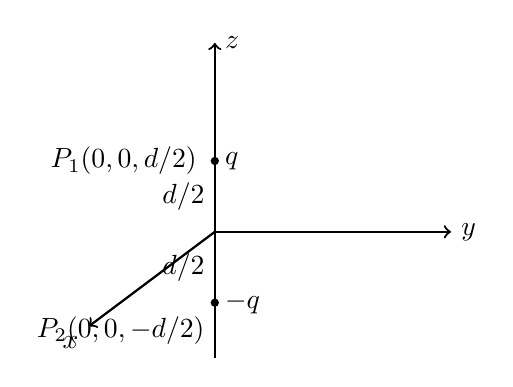
\begin{tikzpicture}[line width=0.8pt]
  \draw[->] (0,-1.6) -- (0,2.4) node[right] {$z$};
  \draw[->] (0,0) -- (3,0) node[right] {$y$};
  \draw[->] (0,0) -- (-1.6,-1.2) node[below left] {$x$};
  \fill (0,0.9) circle (1.5pt) node[right] {$q$};
  \fill (0,-0.9) circle (1.5pt) node[right] {$-q$};
  \node[left] at (-0.1,0.9) {$P_1(0,0,d/2)$};
  \node[below left] at (0,-0.95) {$P_2(0,0,-d/2)$};
  \node[left] at (0,0.45) {$d/2$};
  \node[left] at (0,-0.45) {$d/2$};
\end{tikzpicture}
\end{center}

$p=q\cdot d$ sabit
\begin{align*}
\rho&=q\,\delta(x)\delta(y)\delta(z-d/2)-q\,\delta(x)\delta(y)\delta(z+d/2)\\
&=q\,\delta(x)\delta(y)\left[\frac{\delta(z-d/2)-\delta(z+d/2)}{d}\right]d\\
&=-qd\,\delta(x)\delta(y)\left[\frac{\delta(z+d/2)-\delta(\overbrace{z-d/2}^{z'})}{d}\right]\\
&=-p\,\delta(x)\delta(y)\left[\frac{\delta(z'+d)-\delta(z')}{d}\right]
\end{align*}
\begin{align*}
\rho_{\mathrm{dipol}}&=\lim_{\substack{d\to0\\q\to\infty}}\rho=\lim_{\substack{d\to0\\q\to\infty}}(-p)\,\delta(x)\delta(y)\left[\frac{\delta(z'+d)-\delta(z')}{d}\right]\\
&=-\delta(x)\delta(y)\lim_{\substack{d\to0\\q\to\infty}}p\lim_{\substack{d\to0\\q\to\infty}}\left[\frac{\delta(z'+d)-\delta(z')}{d}\right]\\
&=-\delta(x)\delta(y)\,p\,\delta'(z')\\
\rho_{\mathrm{dipol}}&=-p\,\delta(x)\delta(y)\,\delta'(z-d/2)
\end{align*}

\sayfa{10}
\elcizimi[0.6]{sekiller/final-calismasi-Final-notu-kopya-s10-1.png}[10]

\vurgu{Sonsuz uzun çizgisel yük dağılımı için $\vec E=\dfrac{\rho_c}{2\pi\varepsilon\rho}\,\vec e_\rho$}

\begin{align*}
\vec E&=\frac{-\rho_c}{2\pi\varepsilon\,2a}\,\vec e_x-\frac{\rho_c}{2\pi\varepsilon\,2b}\,\vec e_y\\
&\quad+\frac{\rho_c}{2\pi\varepsilon\,2\sqrt{a^{2}+b^{2}}}\left(\frac{a\,\vec e_x+b\,\vec e_y}{\sqrt{a^{2}+b^{2}}}\right)
\end{align*}
\[
\vec E=\frac{-\rho_c}{4\pi\varepsilon(a^{2}+b^{2})}\left[\vec e_x\frac{b^{2}}{a}+\vec e_y\frac{a^{2}}{b}\right]
\]
\begin{align*}
\vec F&=\int_{z=0}^{z=1}\rho_c\,\vec E\,dz=\rho_c\vec E\\
&=\frac{-\rho_c^{2}}{4\pi\varepsilon(a^{2}+b^{2})}\left[\vec e_x\frac{b^{2}}{a}+\vec e_y\frac{a^{2}}{b}\right]
\end{align*}

\sekilnotu[10]{Bu sayfa basılı materyal içeriyor (sol altta Pr.-8 problem metni, şekil ve $V(M)$ formülü); dijitalleştirilmedi. Şekle elle eklenenler: $M_0$ yanında $(a,b,c)$ ve $M_1$ yanında \textit{görüntü} oku.}

1) Denk problem çözülmeden sınır değerleri yazalım

$z>0$ \quad $\Delta V=\dfrac{-\rho_v}{\varepsilon_1}=\dfrac{-q}{\varepsilon_1}\,\delta(x-a)\delta(y-b)\delta(z-c)$

$z<0$ \quad $\Delta V=0$

$z=0$ sınır problemleri
\begin{gather*}
V_1=V_2\\
\vec n\cdot\vec D_1=\vec n\cdot\vec D_2\\
\vec e_z\cdot\vec D_1=\vec e_z\,\vec D_2
\end{gather*}

$d\to0$'a gidiyordu
\begin{align*}
{\color{kirmizikalem}\star}\ \rho_{z\,\mathrm{dipol}}&=-p\,\delta(x)\delta(y)\delta'(z)\\
\rho_{y\,\mathrm{dipol}}&=-p\,\delta(x)\delta'(y)\delta(z)\\
\rho_{x\,\mathrm{dipol}}&=-p\,\delta'(x)\delta(y)\delta(z)\\
\rho_{\mathrm{dipol}}&=-\operatorname{div}\vec p\\
&=-\operatorname{div}\left[\vec p\,\delta(x-x_0)\delta(y-y_0)\delta(z-z_0)\right]
\end{align*}
\textcolor{kirmizikalem}{örnek $\vec p=p\,\vec e_z$}
\[
=-\operatorname{div}\left[p\vec n\,\delta(x-x_0)\delta(y-y_0)\delta(z-z_0)\right]
\]
\formulkutu{\operatorname{div}(\vec A\cdot f)=f\cdot\operatorname{div}\vec A+\vec A\,\operatorname{grad}f}
\begin{align*}
&=-\delta(x-x_0)\delta(y-y_0)\delta(z-z_0)\,\overset{0}{\operatorname{div}(p\vec n)}\qquad\text{çünkü }\operatorname{div}\vec n=0\\
&\quad-p\vec n\cdot\operatorname{grad}\left[\delta(x-x_0)\delta(y-y_0)\delta(z-z_0)\right]
\end{align*}
\formulkutu{\operatorname{div}\vec e_x=\frac{\partial 1}{\partial x}=0}
\[
\Rightarrow\ \rho_{x\,\mathrm{dipol}}=-p\,\vec e_x\cdot\operatorname{grad}\left[\delta(x-x_0)\delta(y-y_0)\delta(z-z_0)\right]
\]
ve $\operatorname{grad}\left[\delta(x-x_0)\delta(y-y_0)\delta(z-z_0)\right]$
\begin{align*}
&=\delta'(x-x_0)\delta(y-y_0)\delta(z-z_0)\,\vec e_x\\
&\quad+\delta(x-x_0)\delta'(y-y_0)\delta(z-z_0)\,\vec e_y\\
&\quad+\delta(x-x_0)\delta(y-y_0)\delta'(z-z_0)\,\vec e_z
\end{align*}
ve $\vec e_x\cdot\vec e_x=1$ \quad diğerleri $0$
\[
\Rightarrow\ \rho_{x\,\mathrm{dipol}}=-p\,\delta'(x-x_0)\delta(y-y_0)\delta(z-z_0)
\]

\begin{center}
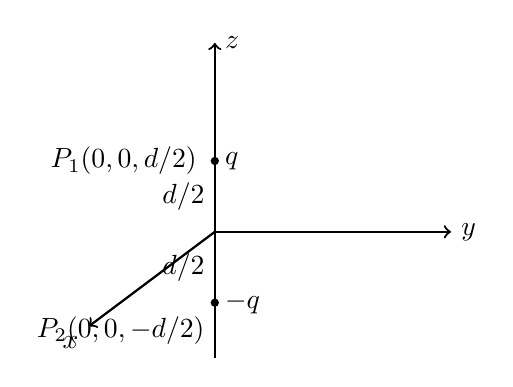
\begin{tikzpicture}[line width=0.8pt]
  \draw[->] (0,-1.6) -- (0,2.4) node[right] {$z$};
  \draw[->] (0,0) -- (3,0) node[right] {$y$};
  \draw[->] (0,0) -- (-1.6,-1.2) node[below left] {$x$};
  \fill (0,0.9) circle (1.5pt) node[right] {$q$};
  \fill (0,-0.9) circle (1.5pt) node[right] {$-q$};
  \node[left] at (-0.1,0.9) {$P_1(0,0,d/2)$};
  \node[below left] at (0,-0.95) {$P_2(0,0,-d/2)$};
  \node[left] at (0,0.45) {$d/2$};
  \node[left] at (0,-0.45) {$d/2$};
\end{tikzpicture}
\end{center}

\[
\rho_{\mathrm{dipol}}=-p\,\vec n\,\operatorname{grad}\left[\delta(x)\delta(y)\delta(z)\right]
\]
\[
V=\frac{1}{4\pi\varepsilon_0}\iiint\frac{\rho_{\mathrm{dipol}}}{r'}\,\underbrace{dv'}_{dx'\,dy'\,dz'}
\]
\[
r'=\sqrt{(x-x')^{2}+(y-y')^{2}+(z-z')^{2}}
\]

\sayfa{11}
Şimdi de denk problem'den bakalım

$z>0$ \quad $\varepsilon_2=\varepsilon_1$ seçelim

\elcizimi[0.65]{sekiller/final-calismasi-Final-notu-kopya-s11-1.png}[11]

M'nin $z>0$ iken M noktasında oluşan potansiyel
\[
V_1=\frac{q}{4\pi\varepsilon_1 r_1}+\frac{\alpha q}{4\pi\varepsilon_1 r_1'}
\]
\[
\vec E_1=-\operatorname{grad}V_1=\frac{q}{4\pi\varepsilon_1}\left(\frac{1}{r_1^{2}}\,\vec e_{r_1}+\frac{\alpha}{r_1'^{2}}\,\vec e_{r_1'}\right)
\]
\begin{align*}
V_1\Big|_{z=0}&=\frac{q}{4\pi\varepsilon_1}\left(\frac1r+\frac{\alpha}{r}\right)\\
&=\frac{q}{4\pi\varepsilon_1 r}\left(\frac1r+\frac{\alpha}{r}\right)\\
&=\frac{q}{4\pi\varepsilon_1 r}\,(1+\alpha)
\end{align*}
\okunamadi{egider}
\[
\vec e_z\cdot\vec D_1\Big|_{z=0}=\frac{q}{4\pi}\left(\frac{\vec e_z\cdot\vec e_{r_1}\big|_{z=0}}{r^{2}}+\alpha\,\frac{\vec e_z\cdot\vec e_{r_1'}\big|_{z=0}}{r^{2}}\right)
\]

\elcizimi[0.62]{sekiller/final-calismasi-Final-notu-kopya-s11-2.png}[11]

\begin{align*}
&=\frac{q}{4\pi r^{2}}\left(-\cos\theta+\alpha\cos\theta\right)\\
&=\kutula{\frac{qc}{4\pi r^{3}}\,(\alpha-1)}
\end{align*}

$z<0$ bölgesinde $\varepsilon_1=\varepsilon_2$ olduğunu varsayarak $M_0$'a bir $q_1$ yükü yerleştirerek denk problemi tanımlayalım

\[
V(x,y,z)=\frac{1}{4\pi\varepsilon_0}\iiint\limits_{x',y',z'=-\infty}^{\infty}\frac{-p\,\vec n\,\operatorname{grad}\left[\delta(x')\delta(y')\delta(z')\right]}{\sqrt{(x-x')^{2}+(y-y')^{2}+(z-z')^{2}}}\,dx'\,dy'\,dz'
\]
{\small
\begin{align*}
V&=\frac{-p\cdot\vec n}{4\pi\varepsilon_0}\Bigg[\vec e_x\iiint\limits_{x',y',z'=-\infty}^{\infty}\frac{\delta'(x')\delta(y')\delta(z')}{\sqrt{(x-x')^{2}+(y-y')^{2}+(z-z')^{2}}}\,dx'dy'dz'\\
&\qquad+\vec e_y\iiint\limits_{x',y',z'=-\infty}^{\infty}\frac{\delta(x')\delta'(y')\delta(z')}{\sqrt{(x-x')^{2}+(y-y')^{2}+(z-z')^{2}}}\,dx'dy'dz'\\
&\qquad+\vec e_z\iiint\limits_{x',y',z'=-\infty}^{\infty}\frac{\delta(x')\delta(y')\delta'(z')}{\sqrt{(x-x')^{2}+(y-y')^{2}+(z-z')^{2}}}\,dx'dy'dz'\Bigg]
\end{align*}
}
\textcolor{turuncukalem}{$\delta(y')f(y')=f(0)\delta(y')$}
{\small
\begin{align*}
V&=\frac{-p\cdot\vec n}{4\pi\varepsilon_0}\Bigg[\vec e_x\iiint\limits_{x',y',z'=-\infty}^{\infty}\frac{\delta'(x')\delta(y')\delta(z')}{\sqrt{(x-x')^{2}+(y)^{2}+(z)^{2}}}\,dx'dy'dz'\\
&\qquad+\vec e_y\iiint\limits_{x',y',z'=-\infty}^{\infty}\frac{\delta(x')\delta'(y')\delta(z')}{\sqrt{(x)^{2}+(y-y')^{2}+(z)^{2}}}\,dx'dy'dz'\\
&\qquad+\vec e_z\iiint\limits_{x',y',z'=-\infty}^{\infty}\frac{\delta(x')\delta(y')\delta'(z')}{\sqrt{(x)^{2}+(y)^{2}+(z-z')^{2}}}\,dx'dy'dz'\Bigg]
\end{align*}
}
\[
{\color{murekkep}\int_{x'=-\infty}^{\infty}\frac{\delta'(x')}{\sqrt{(x-x')^{2}+y^{2}+z^{2}}}\,dx'\cdot\underbrace{\int_{-\infty}^{\infty}\delta(y')\,dy'}_{1}\underbrace{\int_{-\infty}^{\infty}\delta(z')\,dz'}_{1}}
\]
{\small
\begin{align*}
V&=\frac{-p\cdot\vec n}{4\pi\varepsilon_0}\Bigg[\vec e_x\int_{x'=-\infty}^{\infty}\left[(x-x')^{2}+y^{2}+z^{2}\right]^{-1/2}\delta'(x')\,dx'\\
&\qquad+\vec e_y\int_{y'=-\infty}^{\infty}\left[x^{2}+(y-y')^{2}+z^{2}\right]^{-1/2}\delta'(y')\,dy'\\
&\qquad+\vec e_z\int_{z'=-\infty}^{\infty}\left[x^{2}+y^{2}+(z-z')^{2}\right]^{-1/2}\delta'(z')\,dz'\Bigg]
\end{align*}
}
\[
\int_{-\infty}^{\infty}\delta^{(n)}(x-x_0)f(x)=(-1)^{n}f^{(n)}(x_0)
\]
{\small
\begin{align*}
V&=\frac{-p\cdot\vec n}{4\pi\varepsilon_0}\Bigg[\vec e_x\cdot\frac12\cdot\frac{2(x-x')(-1)}{\left[(x-x')^{2}+y^{2}+z^{2}\right]^{3/2}}\Bigg|_{x'=0}\\
&\qquad+\vec e_y\,\frac{(y-y')(-1)}{\left[x^{2}+z^{2}+(y-y')^{2}\right]^{3/2}}\Bigg|_{y'=0}\\
&\qquad+\vec e_z\,\frac{(z-z')(-1)}{\left(x^{2}+y^{2}+(z-z')^{2}\right)^{3/2}}\Bigg|_{z'=0}\Bigg]
\end{align*}
}

\sayfa{12}
\[
V_2=\frac{\beta q}{4\pi\varepsilon_2 r_1'}
\]
\elcizimi[0.47]{sekiller/final-calismasi-Final-notu-kopya-s12-1.png}[12]
\begin{align*}
\vec E&=-\operatorname{grad}V\\
&=-\frac{\partial V}{\partial r}\,\vec e_{r'}\\
&=\frac{\beta q}{4\pi\varepsilon_2 r'^{2}}\,\vec e_{r'}
\end{align*}
\elcizimi[0.45]{sekiller/final-calismasi-Final-notu-kopya-s12-2.png}[12]
$z=0$
\begin{align*}
V_2\Big|_{z=0}&=\frac{\beta q}{4\pi\varepsilon_2 r'}\\
\vec e_z\cdot\vec D_2\Big|_{z=0}&=\frac{\beta q}{4\pi r^{2}}\,\vec e_z\cdot\vec e_{r'}\Big|_{z=0}\\
&=\frac{-\beta q}{4\pi r^{2}}\cos\theta\\
&=\frac{-\beta qc}{4\pi r^{3}}
\end{align*}
\[
V_1\Big|_{z=0}=V_2\Big|_{z=0}
\]
\[
\frac{q}{4\pi\varepsilon_1 r}(1+\alpha)=\frac{\beta q}{4\pi\varepsilon_2 r'}
\]
\[
\kutula{\varepsilon_2(1+\alpha)=\varepsilon_1\beta}
\]
\[
\vec e_z\cdot\vec D_1\Big|_{z=0}=\vec e_z\cdot\vec D_2\Big|_{z=0}
\]
\[
\Rightarrow\ \frac{qc}{4\pi r^{3}}(\alpha-1)=\frac{-\beta qc}{4\pi r^{3}}
\]
\[
(\alpha-1)=-\beta\ \Rightarrow\ \kutula{1-\alpha=\beta}
\]
\begin{align*}
\Rightarrow\ \alpha&=\frac{\varepsilon_1-\varepsilon_2}{\varepsilon_1+\varepsilon_2}\\
\beta&=\frac{2\varepsilon_2}{\varepsilon_1+\varepsilon_2}
\end{align*}
\[
V_1=\frac{q}{4\pi\varepsilon_1 r_1}+\frac{\alpha q}{4\pi\varepsilon_1 r_1'}
\]
\[
V(M)=\begin{cases}V_1,&z>0\\V_2,&z<0\end{cases}=\begin{cases}\dfrac{q}{4\pi\varepsilon_1 r_1}+\dfrac{q(\varepsilon_1-\varepsilon_2)}{4\pi\varepsilon_1(\varepsilon_1+\varepsilon_2)r_1'},&z>0\\[2ex]\dfrac{2q\varepsilon_2}{4\pi\varepsilon_2(\varepsilon_1+\varepsilon_2)r'},&z<0\end{cases}
\]

$z=0$ düzleminde biriken yükü bulalım
\[
\Delta V=\frac{-\rho_v(x,y,z)}{\varepsilon}\qquad V\Big|_{z=0}=V_0
\]

\[
V=\frac{p\vec n}{4\pi\varepsilon_0}\left[\frac{x\vec e_x+y\vec e_y+z\vec e_z}{(x^{2}+y^{2}+z^{2})^{3/2}}\right]=\frac{p\cdot\vec n}{4\pi\varepsilon_0}\left[\frac{\vec r}{r^{3}}\right]
\]
\[
\vec E=-\operatorname{grad}V=-\frac{p}{4\pi\varepsilon_0}\,\vec n\operatorname{div}\left(\frac{\vec r}{r^{3}}\right)
\]
\textcolor{kirmizikalem}{$\operatorname{grad}(\vec a\cdot\vec b)=\vec a\operatorname{div}\vec b+\overset{0}{\vec b\operatorname{div}\vec a}\ \to\ \vec n$}

\elcizimi[0.28]{sekiller/final-calismasi-Final-notu-kopya-s12-3.png}[12]
\[
\vec n=\vec e_z\qquad V=\frac{p\,\vec e_z\cdot\vec r}{4\pi\varepsilon_0 r^{3}}
\]
\begin{align*}
&=\frac{pz}{4\pi\varepsilon_0 r^{3}}\\
&=\frac{pr\cos\theta}{4\pi\varepsilon_0 r^{3}}=\frac{p\cos\theta}{4\pi\varepsilon_0 r^{2}}
\end{align*}
\[
\Delta V=\frac{-\rho}{\varepsilon_0}\qquad\text{poisson denkleminin çözümü}\qquad V=\frac{1}{4\pi\varepsilon_0}\iiint\frac{\rho}{r'}\,dv
\]

\section{Ders 13}
\subsection{Boş uzayda}
$\vec E=-\operatorname{grad}V$ \quad $\vec D=\varepsilon_0\vec E$ \quad $\vec D\parallel\vec E$

\elcizimi[0.25]{sekiller/final-calismasi-Final-notu-kopya-s12-4.png}[12]
\[
\Delta V=\frac{-\rho_{\text{dış}}}{\varepsilon_0}
\]
\[
\operatorname{div}\vec D=\operatorname{div}(\varepsilon_0\vec E)=\rho=\rho_{\text{dış}}
\]

\subsection{Boş olmayan ortam}
\elcizimi[0.55]{sekiller/final-calismasi-Final-notu-kopya-s12-5.png}[12]

Olayları yaratan dış yüklerin yoğunluğu $\rho$ olsun. Zamanla ortamın fiziksel varlığından ötürü iç yükler yerdeğiştirerek belirginleşir ve yarattığı alan $\vec E$'ye katkıda bulunur.

\sekilnotu[12]{Bu sayfa basılı materyal içeriyor (sağ altta kitap metni, (2.16) ve (2.17) bağıntıları; ilk satırları sarı vurgulu); dijitalleştirilmedi.}

\sayfa{13}
\[
V=f(x,y,z)-f(x,y,-z)+V_0
\]
\[
\Delta V=\Delta f(x,y,z)-\overset{0}{\Delta f(x,y,-z)}+\overset{0}{\Delta V_0}
\]
sadece $z>0$ potansiyelin \okunamadi{etkisim}
\[
\rho(x,y,z)=-\varepsilon_1\,\Delta V\big|_{z>0}
\]

\begin{align*}
\operatorname{div}(\varepsilon_0\vec E)&=\rho=\rho_{\text{dış}}+\bar\rho\\
\bar\rho&=-\operatorname{div}\left(\varepsilon_0\chi(\vec E)\vec E\right)
\end{align*}
\begin{align*}
\Rightarrow\ \operatorname{div}(\varepsilon_0\vec E)-\bar\rho&=\rho_{\text{dış}}\\
\operatorname{div}(\varepsilon_0\vec E)+\operatorname{div}(\varepsilon_0\chi(\vec E)\cdot\vec E)&=\rho_{\text{dış}}\\
\operatorname{div}\Big(\varepsilon_0\underbrace{(1+\chi(\vec E))}_{\varepsilon_r>1}\cdot\vec E\Big)&=\rho_{\text{dış}}
\end{align*}
\[
\vec D=\varepsilon_0\varepsilon_r\vec E=\varepsilon\vec E
\]
\[
\Rightarrow\ \operatorname{div}\vec D=\rho_{\text{dış}}=\operatorname{div}(\varepsilon\vec E)
\]
\[
\Delta V=\frac{-\rho_{\text{dış}}}{\varepsilon_0}
\]
\[
\vec E=-\operatorname{grad}V\qquad\vec D=\varepsilon\vec E\qquad\operatorname{rot}\vec E=0
\]
\[
\operatorname{div}\vec D=\rho_{\text{dış}}\qquad\vec F=q\vec E
\]

yüzey üzerinde potansiyel sabitse ve içerde yük yoksa iç bölgede potansiyel sabittir, elektrik alan da sabittir ve içerde $\rho=0$

\subsection{Görüntü kavramı ve yöntemi}
\elcizimi[0.7]{sekiller/final-calismasi-Final-notu-kopya-s13-1.png}[13]
\begin{align*}
\rho_s&=\vec e_z\Big(\vec D_1-\underbrace{\vec D_2}_{0}\Big)\Big|_{z=0}\\
&=\vec e_z\vec D_1\Big|_{z=0}=-\vec e_z\,\varepsilon_1\operatorname{grad}V_1\Big|_{z=0}
\end{align*}

$z<0$ bölgesi ($\varepsilon_2$ dielektrik sabitli \okunamadi{değil})

$V_2=0$ sabit, \quad $\vec E_2=0;\ \vec D_2=0$ \quad $\Big\{$ II.nda bölgede yük olmadığından ve $z=0$ yüzeyi üzerinde $V=0$ sabit olduğundan bölge iletkendir ve potansiyeli $V_2=0$ olur

$z>0$ bölgesi ($\varepsilon_1$ dielektrik sabitli bölge)

$V_1=?$ \quad $\vec E=-\operatorname{grad}V_1$ ; $\vec D_1=\varepsilon_1\vec E_1=-\varepsilon_1\operatorname{grad}V_1$

$\rho=q\,\delta(x-x_0)\delta(y-y_0)\delta(z-z_0)\neq0$

\sayfa{14}
I.nda bölge ise II gibi iletken bir bölge değil $V_1\neq0$

(I) $V_1$'in sağladığı diferansiyel denklem ve sınır koşul dikkate alınmalı.
\[
z>0\text{ da}\ \left\{\begin{array}{l}
\Delta V_1=\dfrac{-\rho}{\varepsilon_1}=\dfrac{-q\,\delta(x-x_0)\delta(y-y_0)\delta(z-z_0)}{\varepsilon_1}\\[1.5ex]
V_1\big|_{z=0}=0\qquad\lim\limits_{z\to\infty}V_1\ \text{için}\ \infty
\end{array}\right.
\]

\textcolor{turuncukalem}{\okunamadi{Eşörnek} problem :} ($z>0$ bölgesi bakımından)

\elcizimi[0.78]{sekiller/final-calismasi-Final-notu-kopya-s14-1.png}[14]
\[
z>0\text{ da}\quad\Delta V_1=\frac{-\rho_1}{\varepsilon_1}=\frac{-q\,\delta(x-x_0)\delta(y-y_0)\delta(z-z_0)}{\varepsilon_1}
\]
\[
V_q\Big|_{z=0}=\frac{q}{4\pi\varepsilon_1 r_1}\qquad V_{-q}\Big|_{z=0}=\frac{-q}{4\pi\varepsilon_1 r_1}
\]
\[
r_1=r_2=\sqrt{z_0^{2}+\ell^{2}}
\]
\textcolor{kirmizikalem}{$\star$ Sadece Tüm uzay homojense \okunamadi{çalan yasış} geçerli}
\[
V\Big|_{z=0}=V_q\Big|_{z=0}+V_{-q}\Big|_{z=0}=0
\]

\elcizimi[0.58]{sekiller/final-calismasi-Final-notu-kopya-s14-2.png}[14]
\[
V_P=\frac{q}{4\pi\varepsilon_1 r_1}-\frac{q}{4\pi\varepsilon_1 r_2}=\frac{q}{4\pi\varepsilon_1}\left(\frac{1}{r_1}-\frac{1}{r_2}\right)
\]
\[
V_P\Big|_{z=0}=0
\]
$z>0$ \quad $V_1=\dfrac{q}{4\pi\varepsilon_1}\left(\dfrac{1}{r_1}-\dfrac{1}{r_2}\right)$

$z<0$ \quad $V_2=0$

\sayfa{15}
\[
\Rightarrow\ \vec E_1=-\operatorname{grad}V_1=\frac{q}{4\pi\varepsilon_1}\left(\frac{\vec r_1}{r_1^{3}}-\frac{\vec r_2}{r_2^{3}}\right)
\]
\[
\vec D_1=\varepsilon_1\vec E_1=\frac{q}{4\pi}\left(\frac{\vec r_1}{r_1^{3}}-\frac{\vec r_2}{r_2^{3}}\right)
\]
\[
\rho_s\Big|_{z=0}=\vec e_z\left(\vec D_1-\vec D_2\right)\Big|_{z=0}=\vec e_z\cdot\vec D_1\Big|_{z=0}
\]
\[
\rho_s=\frac{q}{4\pi}\,\vec e_z\left(\frac{\vec r_1}{r_1^{3}}\Big|_{z=0}-\frac{\vec r_2}{r_2^{3}}\right)\Big|_{z=0}
\]
\[
\vec r_1\Big|_{z=0}=r_1\vec n_1\Big|_{z=0}
\]

\elcizimi[0.72]{sekiller/final-calismasi-Final-notu-kopya-s15-1.png}[15]
\textcolor{turuncukalem}{$|\vec r_1|=|\vec r_2|$}

\textcolor{turuncukalem}{$\vec r_1\neq\vec r_2$}
\begin{align*}
\vec r_1\Big|_{z=0}&=r_1\Big|_{z=0}\vec n_1\Big|_{z=0}=r_1\left[\cos\theta\,\vec e_\ell\footnotemark-\sin\theta\,\vec e_z\right]\\
\vec r_2\Big|_{z=0}&=r_2\Big|_{z=0}\vec n_2\Big|_{z=0}=r_2\left[\cos\theta\,\vec e_\ell+\sin\theta\,\vec e_z\right]
\end{align*}
\footnotetext{Claude notu: İlk birim vektörün alt indisi okunaksız; yatay yön ($\ell$) olarak okundu.}
\[
\rho_s=\frac{q}{4\pi}\,\vec e_z\left(\frac{\vec r_1\big|_{z=0}}{\underbrace{(r_1|_{z=0})^{3}}_{r^{3}}}-\frac{\vec r_2\big|_{z=0}}{\underbrace{(r_2|_{z=0})^{3}}_{r^{3}}}\right)
\]
\begin{align*}
&=\frac{q}{4\pi}\,\frac{\vec e_z}{r^{3}}\left(\vec r_1\big|_{z=0}-\vec r_2\big|_{z=0}\right)\\
&=\frac{q}{4\pi r^{3}}\,\vec e_z\Big[r\cos\theta\,\vec e_\ell-r\sin\theta\,\vec e_z-\\
&\qquad\quad r\cos\theta\,\vec e_\ell-r\sin\theta\,\vec e_z\Big]\\
&=\frac{-q\sin\theta}{2\pi r^{2}}\quad\text{ve}\quad\sin\theta=\frac{\text{karşı}}{\text{hipo}}=\frac{z_0}{r}\\
&=\frac{-qz_0}{2\pi r^{3}}\qquad(\mathrm{C/m^{2}})
\end{align*}
\textcolor{kirmizikalem}{yüzeyin üzerindeki yük 0 değildir ve değişkendir}

\elcizimi[0.8]{sekiller/final-calismasi-Final-notu-kopya-s15-2.png}[15]

\sayfa{16}
\elcizimi[0.3]{sekiller/final-calismasi-Final-notu-kopya-s16-1.png}[16]
$V=\dfrac{q_1}{4\pi\varepsilon r}$ \quad $q_1$ başta vardı, $q_2$ uzaktan getirildi
\[
W=q_2\left(V_1-\underbrace{V_\infty}_{0}\right)=q_2\,\frac{q_1}{4\pi\varepsilon r}
\]
\[
\Rightarrow\ W=\frac12\sum_{i=1}^{n}q_iV_i
\]
3 tane yük var olsun
\begin{align*}
W&=W_{13}+W_{23}+W_{12}\\
&=\frac{q_3q_1}{4\pi\varepsilon r_{13}}+\frac{q_3\cdot q_2}{4\pi\varepsilon r_{23}}+\frac{q_1\cdot q_2}{4\pi\varepsilon r_{12}}
\end{align*}
\elcizimi[0.52]{sekiller/final-calismasi-Final-notu-kopya-s16-2.png}[16]
\textcolor{turuncukalem}{$dv\Rightarrow dq=\rho\,dv$} \quad \textcolor{turuncukalem}{$\rho=\dfrac{dq}{dv}$} \quad $dW=\dfrac12\rho\,dv\cdot V$
\[
W=\frac12\int_v\rho V\,dv=\frac12\int\underbrace{\rho}_{\to\ \operatorname{div}\vec D}V\,dv
\]
\[
=\frac12\int\operatorname{div}\vec D\;V\cdot dv
\]
\[
\vec E=-\operatorname{grad}V=-\frac{\partial V}{\partial n}\,\vec n
\]
\begin{align*}
&=\frac12\int\rho V\,dv=\frac12\int\vec E\cdot\underbrace{\vec D}_{\to\ \varepsilon\vec E}\,dv\\
&=\frac12\int\varepsilon|\vec E|^{2}\,dv
\end{align*}

\subsection{Kapasite problemi}
$C=\dfrac{Q}{V_s}$

\elcizimi[0.22]{sekiller/final-calismasi-Final-notu-kopya-s16-3.png}[16]

\elcizimi[0.46]{sekiller/final-calismasi-Final-notu-kopya-s16-4.png}[16]
\begin{align*}
Q&=C(V_2-V_1)\\
-Q&=C(V_1-V_2)\\
W&=\frac12Q(V_2-V_1)=\frac12\frac{Q^{2}}{C}\\
&=\frac12C(V_2-V_1)^{2}=\frac{\varepsilon}{2d}S(V_1-V_2)^{2}
\end{align*}
$\Rightarrow$ \vurgu{$C=\dfrac{\varepsilon S}{d}$}

\sayfa{17}
\subsection{Bir kürenin kapasitesi}
\elcizimi[0.28]{sekiller/final-calismasi-Final-notu-kopya-s17-1.png}[17]
\[
C=4\pi\varepsilon R
\]

\end{document}
